\documentclass[aspectratio=169, 10pt]{beamer}

\usepackage{bm} % bold math
\usepackage{fontspec}
\usepackage{minted}
\usepackage{pgf-pie}
\usepackage{tikz}
\usepackage{graphicx}
\newcommand\sbullet[1][.5]{\mathbin{\vcenter{\hbox{\scalebox{#1}{$\bullet$}}}}}

% Custom commands and environments
\makeatletter
\newcommand\version[1]{\renewcommand\@version{#1}}
\newcommand\@version{}
\def\insertversion{\@version}

\newcommand\course[1]{\renewcommand\@course{#1}}
\newcommand\@course{}
\def\insertcourse{\@course}

\newcommand\coursetitle[1]{\renewcommand\@coursetitle{#1}}
\newcommand\@coursetitle{}
\def\insertcoursetitle{\@coursetitle}

\newcommand\lecturenumber[1]{\renewcommand\@lecturenumber{#1}}
\newcommand\@lecturenumber{}
\def\insertlecturenumber{\@lecturenumber}
\makeatother

\newcommand{\slidetitle}[1]{{\xbseries \large \structure{#1}} \bigskip}
\newcommand{\term}[1]{{\color{blue} #1}}
\newcommand{\leftspace}{\hspace{1em}}
\newcommand{\inlinearrow}{
  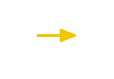
\begin{tikzpicture}[baseline]
    \node [anchor=base] (x) {};
    \draw [rawarrow] (x.mid west) -- ($(x.mid west) + (2em,0)$);
  \end{tikzpicture}
}

\newenvironment{slide}
{\begin{frame}[fragile,environment=slide]\vskip0pt plus 1filll}
{\vskip0pt plus 1filll\end{frame}}

% LaTeX

\setlength{\leftmargini}{1em}

% Common Information

\author{Talia Xu}
\course{COMPSCI 340}
\coursetitle{Operating Systems}
\date{2024 Semester 2}

% fontspec

\defaultfontfeatures{Ligatures=TeX}
% \setmainfont{Domine}
\setsansfont{Inter}[
  FontFace={ul}{n}{Font=*-Thin},
  FontFace={el}{n}{Font=*-ExtraLight},
  FontFace={l}{n}{Font=*-Light},
  FontFace={sb}{n}{Font=*-SemiBold},
  FontFace={eb}{n}{Font=*-ExtraBold},
  FontFace={xb}{n}{Font=*-Black},
]
\setmonofont[Contextuals=AlternateOff, Ligatures=TeXOff]{Iosevka}[
  FontFace={xb}{n}{Font=*-Heavy},
]

%% Font Weights

\DeclareRobustCommand{\ulseries}{\fontseries{ul}\selectfont}
\DeclareTextFontCommand{\textul}{\ulseries}
\DeclareRobustCommand{\elseries}{\fontseries{el}\selectfont}
\DeclareTextFontCommand{\textel}{\elseries}
\DeclareRobustCommand{\lseries}{\fontseries{l}\selectfont}
\DeclareTextFontCommand{\textl}{\lseries}
\DeclareRobustCommand{\sbseries}{\fontseries{sb}\selectfont}
\DeclareTextFontCommand{\textsb}{\sbseries}
\DeclareRobustCommand{\ebseries}{\fontseries{eb}\selectfont}
\DeclareTextFontCommand{\texteb}{\ebseries}
\DeclareRobustCommand{\xbseries}{\fontseries{xb}\selectfont}
\DeclareTextFontCommand{\textxb}{\xbseries}

% tikz

\usetikzlibrary{
  arrows,
  arrows.meta,
  automata,
  backgrounds,
  calc,
  decorations.pathreplacing,
  matrix,
  positioning,
  overlay-beamer-styles,
  shapes,
  shapes.multipart,
  tikzmark,
}

\tikzstyle{rawarrow} = [
  -{Latex[round]},
  line width=1pt,
  yellow,
  shorten >=3pt,
  shorten <=3pt,
  font=\small,
  text=black,
]

\tikzstyle{arrow} = [
  -{Latex[round]},
  line width=1pt,
  yellow,
  shorten >=3pt,
  shorten <=3pt,
  transform canvas={yshift=3pt},
  font=\small,
  text=black,
]

\newcommand{\tikzmarkcoord}[1]{([yshift=3pt]pic cs:#1)}

% minted

\setminted{style=eyolfson, fontsize=\small, escapeinside=||}
\setmintedinline{fontsize=\normalsize}

% hyperref

\hypersetup{colorlinks, urlcolor=blue}

% beamer
\setbeamersize{text margin left=16mm, text margin right=16mm}
\setbeamertemplate{itemize items}[circle]
\setbeamercolor{item}{fg=black}
\setbeamercolor{structure}{fg=darkblue}
\setbeamerfont{frametitle}{series=\bfseries, parent=structure}
\setbeamertemplate{navigation symbols}{}
\setbeamertemplate{headline}{}
\setbeamertemplate{footline}{
  \begin{tikzpicture}[
    remember picture,
    overlay,
    shift={(current page.south west)},
  ]
    \path [fill=gray] (144mm, 0) -- (160mm, 16mm) -- (160mm, 0);
    \node [inner sep=3.5mm, outer sep=0, text=black, anchor=base east,
           align=right, yshift=3.5mm]
          at (current page.south east) {\ttfamily \small \insertframenumber{}};
  \end{tikzpicture}
}
\setbeamertemplate{title page}{
  \begin{tikzpicture}[
    remember picture,
    overlay,
    shift={(current page.south west)},
    background rectangle/.style={fill=darkblue},
    show background rectangle,
  ]
    \node [anchor=center, align=center, text=white, text width=40mm, scale=3.2]
          at (\paperwidth / 2, \paperheight * 2 / 3)
          {\xbseries \inserttitle{}};
    \node [anchor=base west, align=left, inner sep=0, text=white, yshift=2.5mm]
          at (16mm, \paperheight / 3)
          {\insertdate{} \insertcourse{}: \insertcoursetitle{}};
    \node [anchor=base west, align=left, inner sep=0, text=white, yshift=-2.5mm]
          at (16mm, \paperheight / 3)
          {\insertauthor};
    \node [anchor=base east, align=right, inner sep=0, text=white, yshift=2.5mm]
          at (144mm, \paperheight / 3)
          {Lecture \insertlecturenumber{}};
    \node [anchor=base east, align=right, inner sep=0, text=white,
           yshift=-2.5mm]
          at (144mm, \paperheight / 3)
          {\ttfamily \insertversion{}};
    \node [align=center, anchor=south, inner sep=0, text=white, yshift=3.5mm]
          (license) at (\paperwidth / 2, 0)
          {\fontsize{7pt}{7pt}\selectfont This  work is licensed under a
           \href{http://creativecommons.org/licenses/by-sa/4.0/}
                {\color{lightblue} Creative Commons Attribution-ShareAlike 4.0
                 International License}};
  \end{tikzpicture}
}

% xcolor

%% Primary Colour

\definecolor{pantone655}{RGB}{0, 42, 92} % #002a5c
\colorlet{darkblue}{pantone655}

%% Secondary Colours

\definecolor{pantone633}{RGB}{0, 139, 176} % #008bb0
\colorlet{blue}{pantone633}

\definecolor{pantonewarmred}{RGB}{220, 70, 51} % #dc4633
\colorlet{red}{pantonewarmred}

\definecolor{pantone3285}{RGB}{0, 161, 137} % #00a189
\colorlet{cyan}{pantone3285}

\definecolor{pantone7722}{RGB}{13, 83, 77} % #0d534d
\colorlet{darkcyan}{pantone7722}

\definecolor{pantone376}{RGB}{141, 191, 46} % #8dbf2e
\colorlet{green}{pantone376}

\definecolor{pantone2613}{RGB}{109, 36, 122} % #6d247a
\colorlet{violet}{pantone2613}

\definecolor{pantone2985}{RGB}{111, 199, 234} % #6fc7ea
\colorlet{lightblue}{pantone2985}

\definecolor{pantone227}{RGB}{171, 19, 104} % #ab1368
\colorlet{magenta}{pantone227}

\definecolor{pantone7406}{RGB}{241, 197, 0} % #f1c500
\colorlet{yellow}{pantone7406}

%% Neutrals

\definecolor{pantonecoolgray2}{RGB}{208, 209, 201} % #d0d1c9
\colorlet{gray}{pantonecoolgray2}


\lecturenumber{6}
\title{Basic IPC}
\version{2.0.0}

\begin{document}

  \begin{frame}[plain, noframenumbering]
    \titlepage
  \end{frame}

  \begin{slide}

    \slidetitle{IPC is Transferring Bytes Between Two or More Processes}

    Reading and writing files is a form of IPC
    \medskip

    The read and write system calls allow any bytes

  \end{slide}

  \begin{slide}

    \slidetitle{A Simple Process Could Write Everything It Reads}

    See: \texttt{06-basic-ipc/read-write-example.c}
    \medskip

    We \texttt{read} from standard in, and \texttt{write} to standard out

    \leftspace{}Does this remind you of any program you've seen before?
    \medskip

    If we run it in our terminal without arguments, it'll wait for input

    \leftspace{}Press Ctrl+D when you're done to send end-of-file (EOF)
  \end{slide}

  \begin{slide}
    \slidetitle{\texttt{\bfseries read} Just Reads Data from a File Descriptor}

    See: \texttt{man 2 read}
    \medskip

    There's no EOF character, \texttt{read} just returns 0 bytes read

    \leftspace{}The kernel returns 0 on a closed file descriptor
    \medskip

    We need to check for errors!

    \leftspace{}Save \texttt{errno} if you're using another function that may
                  set it

  \end{slide}

  \begin{slide}

    \slidetitle{\texttt{\bfseries write} Just Writes Data to a File Descriptor}

    See: \texttt{man 2 write}
    \medskip

    It returns the number of bytes written, you can't assume it's always
    successful

    \leftspace{}Save \texttt{errno} if you're using another function that may
                  set it
    \medskip

    Both ends of the read and write have a corresponding write and read

    \leftspace{}This makes two communication channels with command line programs

  \end{slide}

  \begin{slide}

    \slidetitle{The Standard File Descriptors Are Powerful}

    We could close standard input (freeing file descriptor 0) and open a file
    instead

    \leftspace{}Linux uses the lowest available file descriptor for new ones
    \medskip

    See: \texttt{lecture-06/open-example.c} and \texttt{man 2 open}
    \medskip

    Without changing the core code, it now works with multiple input types

    \leftspace{}You could type, or use a file

  \end{slide}

  \begin{slide}

    \slidetitle{Your Shell Will Let You Redirect Standard File Descriptors}

    Instead of running \texttt{./open-example open-example.c} we could run:

    \leftspace{}\texttt{./open-example < open-example.c}
    \medskip

    Your shell will do the \texttt{open} for you and replace the standard input

    \leftspace{}We didn't actually have to write that!
    \medskip

    You could also redirect across multiple processes

    \leftspace{}\texttt{cat open-example.c | ./open-example} 

  \end{slide}

  \begin{slide}

    \slidetitle{Signals are a Form of IPC that Interrupts}

    You could also press Ctrl+C to stop \texttt{./open-example}

    \leftspace{}This interrupts your programs execution and exits early
    \medskip

    Kernel sends a number to your program indicating the type of signal

    \leftspace{}Kernel default handlers either ignore the signal or terminate
    your process
    \medskip

    Ctrl+C sends \texttt{SIGINT} (interrupt from keyboard)
    \medskip

    If the default handler occurs the exit code will be 128 + signal number

  \end{slide}

  \begin{slide}

    \slidetitle{You Can Set Your Own Signal Handlers with \texttt{sigaction}}

    See: \texttt{06-basic-ipc/signal-example.c} and \texttt{man 2 sigaction}
    \medskip

    You just declare a function that doesn't return a value, and has an \texttt{int} argument

    \leftspace{}The integer is the signal number
    \medskip

    Some numbers are non-standard, below are a few from Linux x86-64:
    \begin{itemize}
      \item 2: \texttt{SIGINT} (interrupt from keyboard)
      \item 9: \texttt{SIGKILL} (terminate immediately)
      \item 11: \texttt{SIGSEGV} (memory access violation)
      \item 15: \texttt{SIGTERM} (terminate)
    \end{itemize}

  \end{slide}

  \begin{slide}
    \slidetitle{A Signal Pauses Your Process and Runs the Signal Handler}

    Your process can be interrupted at any point in execution

    \leftspace{}Your process resumes after the signal handler finishes
    \medskip

    This is an example of concurrency, your process switches execution

    \leftspace{}You have to be careful what you write here
    \medskip

    Run \texttt{./signal-example} and press Ctrl+C

  \end{slide}

  \begin{slide}

    \slidetitle{You Need to Account for Interrupted System Calls}

    You should see:

    \leftspace{}\texttt{Ignoring signal 2}

    \leftspace{}\texttt{read: Interrupted system call}
    \medskip

    We can rewrite it to retry interrupted system calls

    \leftspace{}See: \texttt{06-basic-ipc/signal-example-2.c}
    \medskip

    Now the program continues when we press Ctrl+C

  \end{slide}

  \begin{slide}

    \slidetitle{You Can Send Signals to Processes with Their PID}

    You can use the command: \texttt{kill}

    \leftspace{}It is also a system call, taking a \texttt{pid} and signal number
    \medskip

    Find a processes' ID with \texttt{pidof}, e.g. \texttt{pidof ./signal-example-2}
    \medskip

    After use \texttt{kill <pid>}, which by default sends \texttt{SIGTERM}
    \medskip

    Use \texttt{kill -9 <pid>} to tell the kernel to terminate the process

    \leftspace{}Process won't terminate if it's in uninterruptible sleep

  \end{slide}

  \begin{slide}

    \slidetitle{Most Operations Are Non-Blocking}

    A non-blocking call returns immediately, and you check if something occurs
    \medskip

    To turn \texttt{wait} into a non-blocking call, use \texttt{waitpid} with
    \texttt{WNOHANG} in \texttt{options}
    \medskip

    To react to changes to a non-blocking call, we can either use a
    \textit{poll} or \textit{interrupt}

  \end{slide}

  \begin{slide}

    \slidetitle{Polling Continuously Calls the Function and Checks for Changes}

    See: \texttt{06-basic-ipc/wait-poll-example.c}
    \medskip

    We call \texttt{waitpid} over and over until the child exits

    \leftspace{}Note: some hardware behaves like this,

    \leftspace{}\leftspace{}the kernel may have to check for changes
    \bigskip

    What's the drawback of this approach?

  \end{slide}

  \begin{slide}

    \slidetitle{An Interrupt Instead Occurs Right After the Change}

    See: \texttt{06-basic-ipc/wait-interrupt-example.c}
    \medskip

    Instead of calling \texttt{wait} or \texttt{waitpid} from \texttt{main},
    we can do it in the interrupt handler

    \leftspace{}The kernel sends the \texttt{SIGCHLD} whenever one of its
                  children exit
    \medskip

    This idea also applies to the kernel, hardware can generate interrupts

  \end{slide}

  \begin{slide}

    \slidetitle{Interrupt Handlers Run to Completion}

    See: \texttt{06-basic-ipc/signal-close-example.c}
    \medskip

    An interrupt may occur while an interrupt handler is already running
    \bigskip

    All interrupt handler code must be reentrant

    \leftspace{}You need to be able to pause execution,

    \leftspace{}execute another call (to the same function),

    \leftspace{}and resume execution

  \end{slide}

  \begin{slide}

    \slidetitle{On a RISC-V CPU, There's 3 Terms for ``Interrupts''}

    \textit{Interrupt}

    \leftspace{}Triggered by external hardware,

    \leftspace{}handled by the kernel (needs to respond quickly)
    \bigskip

    \textit{Exception}

    \leftspace{}Triggered by an instruction (divide by zero, illegal memory
                  access),

    \leftspace{}default handler is the kernel (calling process suspended),

    \leftspace{}the process can optionally handle some of these themselves
    \bigskip

    \textit{Trap}

    \leftspace{}Transfer of control to a trap handler caused by either

    \leftspace{}an exception or an interrupt (code that runs)
    \medskip

    A system call would be a \textit{requested trap}
  \end{slide}

  \begin{slide}

    \slidetitle{We Explored Basic IPC in an Operating System}

    Some basic IPC includes:
    \begin{itemize}
      \item \texttt{read} and \texttt{write} through file descriptors (could be a regular file)
      \item Redirecting file descriptors for communcation
      \item Signals
    \end{itemize}
    \medskip

    Signals are like interrupts for user processes

    \leftspace{}The kernel has to handle all 3 kinds of ``interrupts''

  \end{slide}

\end{document}
